
\section{Heuristic generation with \our{}}\label{sec: heuristic generation}

This section presents novel applications of LHH across heterogeneous algorithmic types and diverse COPs. With \our{}, we yield state-of-the-art and competitive meta-heuristics, evolutionary algorithms, heuristics, and neural solvers. 
% \red{We also discuss the rationale behind our experimental setup in \cref{app: further discussions}.}


Hyperparameters of \our{} and detailed experimental setup are given in \cref{app: problem settings}.
We apply \our{} to different algorithmic types across six diverse COPs representative of different areas:
Traveling Salesman Problem (TSP), Capacitated Vehicle Routing Problem (CVRP), and Orienteering Problem (OP) for routing problems; Multiple Knapsack Problem (MKP) for subset problems; Bin Packing Problem (BPP) for grouping problems; and Decap Placement Problem (DPP) for electronic design automation (EDA) problems. Details of the benchmark COPs are given in \cref{app: benchmark problems}. The best \our{}-generated heuristics are collected in \cref{app: generated heuristics}.



\subsection{Penalty heuristics for Guided Local Search}

We evolve penalty heuristics for Guided Local Search (GLS) \cite{arnold2019_KGLS_VRP}. GLS interleaves local search with solution perturbation. The perturbation is guided by the penalty heuristics to maximize its utility. \our{} searches for the penalty heuristic that leads to the best GLS performance.

We implement the best heuristic generated by \our{} within KGLS \cite{arnold2019_KGLS_VRP} and refer to such coupling as KGLS-\our{}. In \cref{tab: main-exp-gls}, we compare KGLS-\our{} with the original KGLS, other GLS variants \cite{hudson2022_gnn_gls, sui2023neuralgls, liu2024_llm_gls}, and SOTA NCO method that learns to improve a solution \cite{ma2023neu_kopt}. The results show that \our{} can improve KGLS and outperform SOTA baselines. In addition, we use a single heuristic for TSP20 to 200, while NCO baselines require training models specific to each problem size.





\begin{table}[h]
    \caption{Evaluation results of different local search (LS) variants. We report optimality gaps and per-instance execution time.}
    \label{tab: main-exp-gls}
    \resizebox{\textwidth}{!}{
    \begin{tabular}{c|c|cc|cc|cc|cc}
    \toprule
    \multirow{2}{*}{Method} & \multirow{2}{*}{Type} & \multicolumn{2}{c|}{TSP20} & \multicolumn{2}{c|}{TSP50} & \multicolumn{2}{c|}{TSP100} & \multicolumn{2}{c}{TSP200} \\
                            &                       & Opt. gap (\%)  & Time (s) & Opt. gap (\%)  & Time (s) & Opt. gap (\%)  & Time (s)  & Opt. gap (\%)  & Time (s)  \\
    \midrule
    NeuOpt* \cite{ma2023neu_kopt} & LS+RL & 0.000  & 0.124  & 0.000 & 1.32 & 0.027 & 2.67  & 0.403  & 4.81      \\
    GNNGLS \cite{hudson2022_gnn_gls}   & GLS+SL  & 0.000 & 0.116  & 0.052 & 3.83  & 0.705 & 6.78  & 3.522   & 9.92      \\
    NeuralGLS{\dag} \cite{sui2023neuralgls}  & GLS+SL  & 0.000 & 10.005 & 0.003 & 10.01 & 0.470 & 10.02 & 3.622 & 10.12 \\
    EoH \cite{liu2024_llm_gls}     & GLS+LHH & 0.000 & 0.563    & 0.000 & 1.90    & 0.025 & 5.87    & 0.338     & 17.52      \\ \midrule
    KGLS{\ddag} \cite{arnold2019_KGLS_VRP}    & GLS     &  0.004     &    0.001    &   0.017    &   0.03     &  0.002     &   1.55     &    0.284   &     2.52   \\
    KGLS-\our{}{\ddag} & GLS+LHH &   \textbf{0.000}    &     \textbf{0.001}   &   \textbf{0.000}    &    \textbf{0.03}    &   \textbf{0.000}    &   \textbf{1.55}     &  \textbf{0.216}     &   \textbf{2.52}     \\
    \bottomrule
    \multicolumn{10}{l}{*: All instances are solved in one batch. D2A=1; T=500, 4000, 5000, and 5000 for 4 problem sizes, respectively.}  \\
    \multicolumn{10}{l}{\dag: The results are drawn from the original literature. \ddag: They are based on our own GLS implementation.}  
    \end{tabular}}
    \end{table}
    
    

\subsection{Heuristic measures for Ant Colony Optimization}\label{sec: heuristic measures for aco}

Solutions to COPs can be stochastically sampled, with heuristic measures indicating the promise of solution components and biasing the sampling. Ant Colony Optimization (ACO), which interleaves stochastic solution sampling with pheromone update, builds on this idea. We generate such heuristic measures for five different COPs: TSP, CVRP, OP, MKP, and BPP.

Under the ACO framework, we evaluate the best \our{}-generated heuristics against the expert-designed ones and neural heuristics specifically learned for ACO \cite{ye2023deepaco}. The evolution curves displayed in \cref{fig: aco-evolution-curves} verify the consistent superiority of \our{} across COPs and problem sizes. Notably, on 3 out of 5 COPs, \our{} outperforms DeepACO \cite{ye2023deepaco} even when the latter overfits the test problem size (TSP50, OP50, and MKP100). We observe that most \our{}-generated heuristics show consistent performance across problem sizes and distributions. Hence, their advantages grow as the distributional shift increases for neural heuristics.



\begin{figure*}[!t]
    \centering
    \begin{minipage}[t]{0.17\textwidth} 
        \centering
        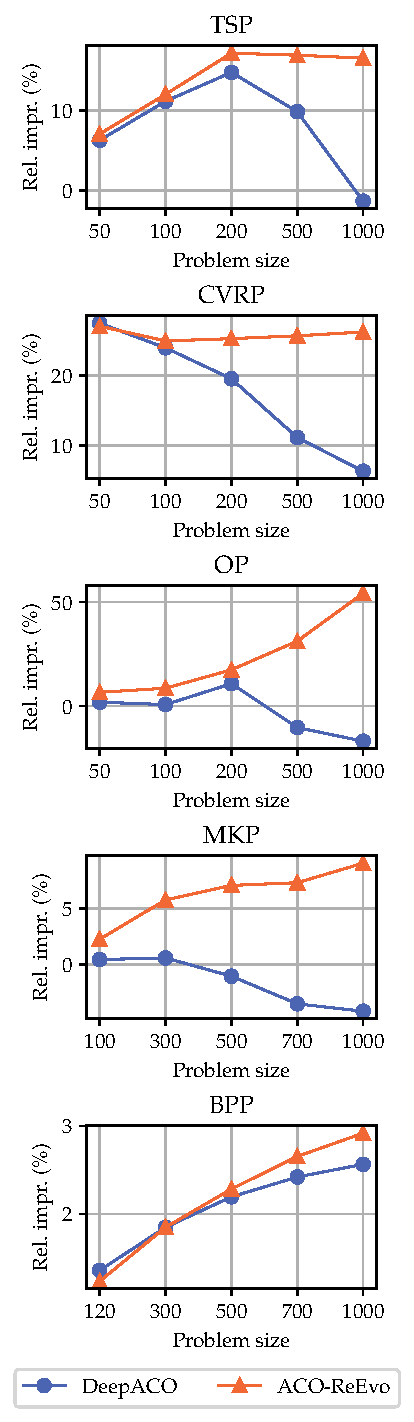
\includegraphics[width=\linewidth]{figures/reevo_aco_exp_improvement.pdf}
    \end{minipage}
    \hfill
    \begin{minipage}[t]{0.81\textwidth}
        \centering
        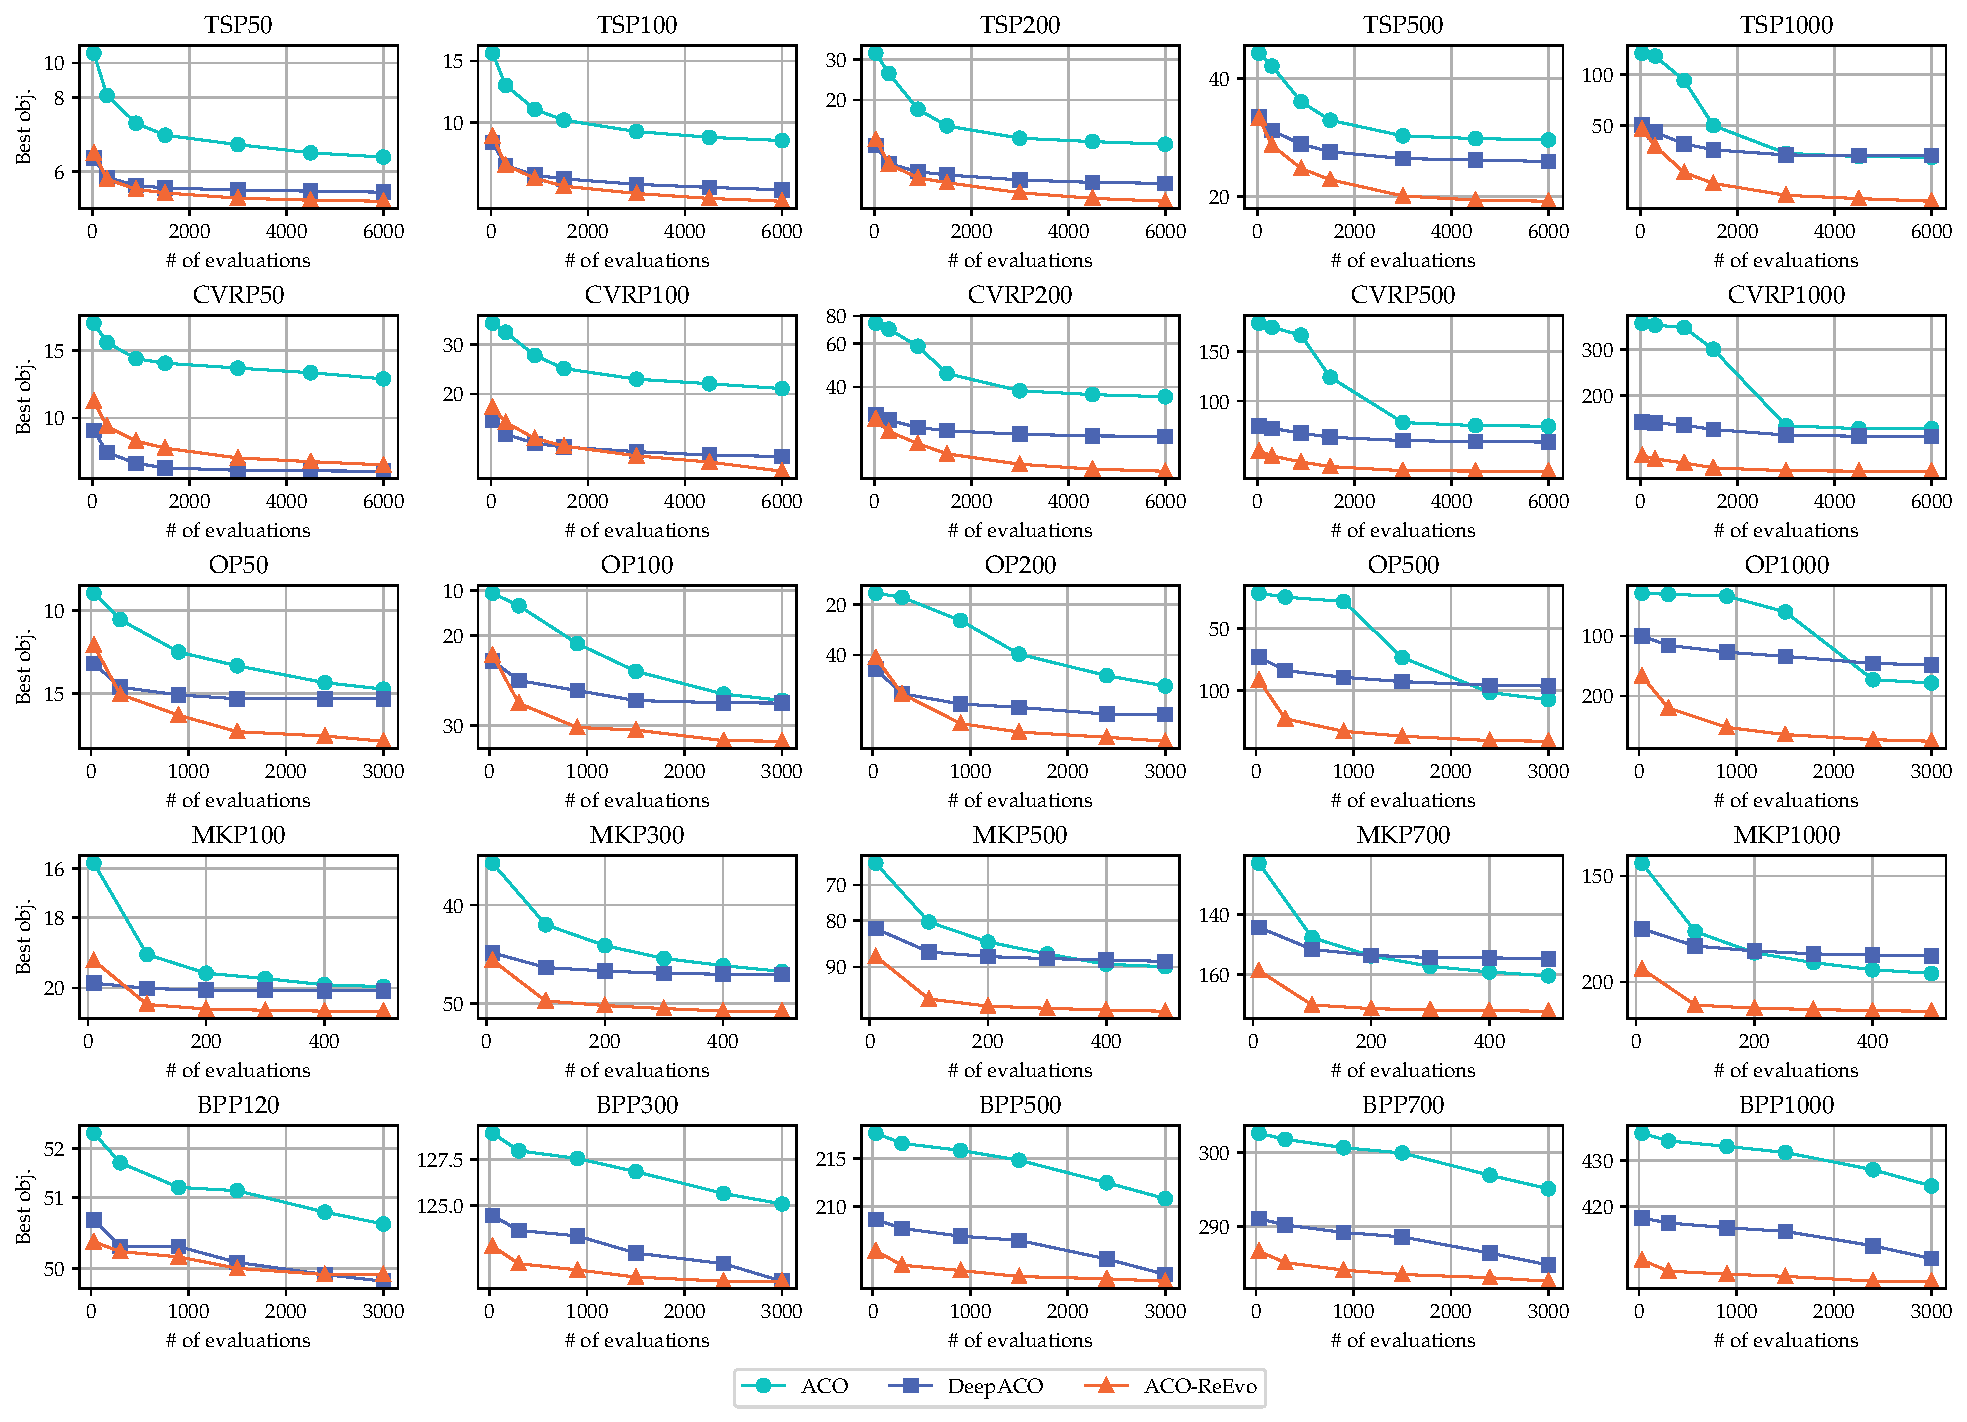
\includegraphics[width=\linewidth]{figures/reevo_aco_exp.pdf}
    \end{minipage}
    \caption{Comparative evaluations of ACO using expert-designed heuristics \cite{skinderowicz2022_aco_tsp_human_bl, cai2022_aco_cvrp_human_bl, sohrabi2021_aco_op_human_bl, fidanova2020_aco_mkp_human_bl, levine2004_aco_bpp_human_bl}, neural heuristics \cite{ye2023deepaco}, and \our{} heuristics. For each COP, the same neural heuristic or the \our{} heuristic is applied across all problem sizes; both heuristics are trained exclusively on the smallest problem size among the five. \textbf{Left}: Relative performance improvement of DeepACO and \our{} over human baselines w.r.t. problem sizes. \textbf{Right}: ACO evolution curves, plotting the all-time best objective value w.r.t. the number of solution evaluations. The curves are averaged over three runs in which only small variances are observed (e.g., $\sim 0.01$ for TSP50).}
    \label{fig: aco-evolution-curves}
\end{figure*}




\subsection{Genetic operators for Electronic Design Automation}

Expert-designed GAs are widely adopted in EDA \cite{shibasaka2013decoupling, zebulum2018evolutionary_electronics, de2020genetic, jiang2024novel}. Besides directly solving EDA problems, GA-generated solutions can be used to train amortized neural solvers \cite{kim2023devformer}. Here, we show that \our{} can improve the expert-designed GAs and outperform DevFormer \citep{kim2023devformer}, the SOTA solver for the DPP problem. We sequentially evolve with \our{} the crossover and mutation operators for the GA expert-designed by \citet{park2023versatile}. \cref{fig:dpp-fig-tab} compares online and offline learned methods, DevFormer, the original expert-designed GA, and the GA with \our{}-generated operators, showing that the \our{}-designed GA outperforms previous methods and, importantly, both the expert-designed GA and DevFormer.




\noindent % Ensures no indentation for alignment
\begin{figure}[b]
  \centering % Centering figure
  \begin{minipage}{0.48\textwidth}
    \centering
    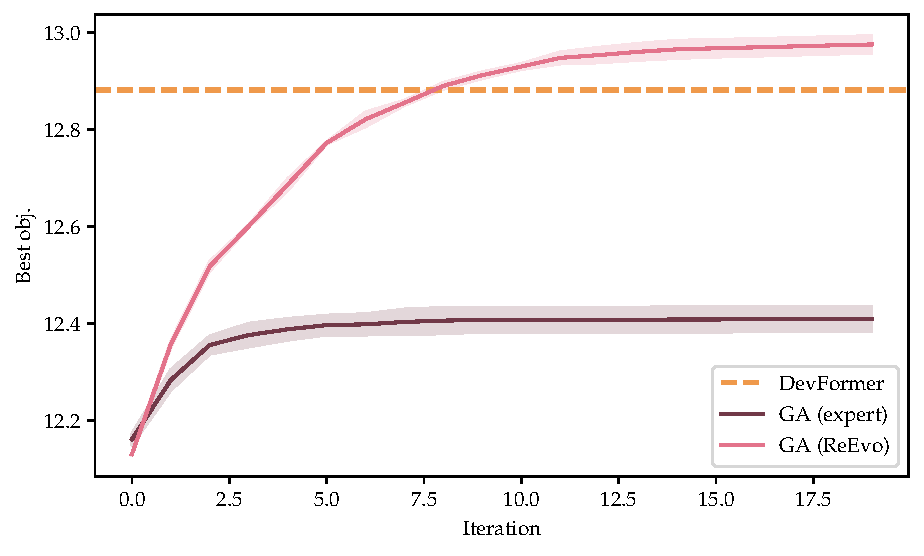
\includegraphics[height=4cm]{figures/dpp_plot.pdf} % Set the height of the figure
    % Caption and label can be omitted here
  \end{minipage}
  \hfill % Space between the minipages
  \begin{minipage}{0.42\textwidth}
    \centering
    \vspace{-.4cm} % Ensures the top alignment affects the table correctly
    \resizebox{\linewidth}{!}{% Resize table to fit the minipage width
    \begin{tabular}{lcc}
        \toprule 
        Method  & \# of shots & Obj. $\uparrow$ \\
        \midrule
        Pointer-PG \cite{kim2021_Pointer-PG-CRL} & 10,000 & 9.66 \tiny $\pm$ 0.206\\
        AM-PG \cite{park2020_AM-PG} & 10,000 & 9.63 \tiny $\pm$ 0.587\\
        CNN-DQN \cite{park2020_CNN-DQN} & 10,000 & 9.79 \tiny $\pm$ 0.267\\
        CNN-DDQN \cite{zhang2020_CNN-DDQN} & 10,000 & 9.63 \tiny $\pm$ 0.150\\
        Pointer-CRL \cite{kim2021_Pointer-PG-CRL} & Zero Shot & 9.59 \tiny $\pm$ 0.232\\
        AM-CRL \cite{park2022_AM-CRL}  & Zero Shot & 9.56 \tiny $\pm$ 0.471\\
        DevFormer-CSE \cite{kim2023devformer} & Zero Shot & 12.88 \tiny $\pm$ 0.003\\
        \midrule
        GA-expert  \cite{park2023versatile}  & 400 & 12.41 \tiny $\pm$ 0.026 \\
        GA-\our{} (ours) & 400 &  \textbf{12.98 \tiny $\pm$ 0.018} \\
        \bottomrule
    \end{tabular}}
    % Caption and label can be omitted here
  \end{minipage}
  \vspace{-3mm} % adjust spacing
  \caption{\textbf{Left}: Comparison of DevFormer \cite{kim2023devformer}, the expert-designed GA \cite{park2023versatile} and our \our{}-designed GA on DPP. The evolution curves plot the best objective value over generations; the horizontal line indicates the reward of end-to-end solutions generated by DevFormer. \textbf{Right}: Evaluation results of DPP solvers. We report the number of solution generations and the average objective value of 100 test problems.}
   \label{fig:dpp-fig-tab}
\end{figure}


\subsection{Constructive heuristics for the Traveling Salesman Problem}

Heuristics can be used for deterministic solution construction by sequentially assigning values to each decision variable. We evaluate the constructive heuristic for TSP generated by \our{} on real-world benchmark instances from TSPLIB \citep{reinelt1991tsplib} in \cref{tab: exp-cons-tsp-ghpp}. \our{} can generate better heuristics than GHPP \cite{duflo2019gp_hh_tsp}, a classic HH based on GP.


\begin{table}[!h]
    \centering
    \footnotesize
    \caption{Comparisons of constructive heuristics designed by human, GHPP \cite{duflo2019gp_hh_tsp}, and \our{}. We report the average optimality gap of each instance, where the baseline results are drawn from \cite{duflo2019gp_hh_tsp} and the results of \our{} are averaged over 3 runs with different starting nodes.} \label{tab: exp-cons-tsp-ghpp}
    \resizebox{0.47\textwidth}{!}{
    \begin{tabular}{l|ccc}
    \toprule
    \multicolumn{1}{c|}{Instance} & Nearest Neighbour & GHPP \cite{duflo2019gp_hh_tsp} & \our{} \\ \midrule
    ts225                         & 16.8  & 7.7 & \textbf{6.6}  \\
    rat99                         & 21.8  & 14.1 & \textbf{12.4}  \\
    rl1889                        & 23.7  & 21.1 & \textbf{17.5}  \\
    u1817                         & 22.2  & 21.2 & \textbf{16.6}  \\
    d1655                         & 23.9  & 18.7 & \textbf{17.5}  \\
    bier127                       & 23.3  & 15.6 & \textbf{10.8}  \\
    lin318                        & 25.8  & \textbf{14.3} &  16.6 \\
    eil51                         & 32.0  & 10.2 & \textbf{6.5}  \\
    d493                          & 24.0  & 15.6 & \textbf{13.4}  \\
    kroB100                       & 26.3  & 14.1 & \textbf{12.2}  \\
    kroC100                       & 25.8  & 16.2 & \textbf{15.9}  \\ \bottomrule
    \end{tabular}}
    \hfill
    \resizebox{0.49\textwidth}{!}{
    \begin{tabular}{l|ccc}
    \toprule
    \multicolumn{1}{c|}{Instance} & Nearest Neighbour & GHPP \cite{duflo2019gp_hh_tsp} & \our{} \\ \midrule
    ch130                         & 25.7  & 14.8 & \textbf{9.4}  \\
    pr299                         & 31.4  & \textbf{18.2} & 20.6  \\
    fl417                         & 32.4  & 22.7 & \textbf{19.2}  \\
    d657                          & 29.7  & 16.3 & \textbf{16.0}  \\
    kroA150                       & 26.1  & 15.6 & \textbf{11.6}  \\
    fl1577                        & 25.0  & 17.6 & \textbf{12.1}  \\
    u724                          & 28.5  & \textbf{15.5} & 16.9  \\
    pr264                         & 17.9  & 24.0 & \textbf{16.8}  \\
    pr226                         & 24.6  & \textbf{15.5} & 18.0  \\
    pr439                         & 27.4  & 21.4 & \textbf{19.3}  \\ \midrule
    Avg. opt. gap                 & 25.4  & 16.7 & \textbf{14.6}  \\ \bottomrule
    \end{tabular}}
\end{table}



\subsection{Attention reshaping for Neural Combinatorial Optimization}\label{sec: attention reshaping for nco}
% Introduction
Autoregressive NCO solvers suffer from limited scaling-up generalization \cite{joshi2020_learning_tsp_requires_rethinking_generalization}, partially due to the dispersion of attention scores \cite{wang2024distance_aware_attention_reshaping}. \citet{wang2024distance_aware_attention_reshaping} design a distance-aware heuristic to reshape the attention scores, which improves the generalization of NCO solvers without additional training. However, the expert-designed attention-reshaping can be suboptimal and does not generalize across neural models or problem distributions.


Here we show that \our{} can automatically and efficiently tailor attention reshaping for specific neural models and problem distributions of interest.
We apply attention reshaping designed by experts \cite{wang2024distance_aware_attention_reshaping} and \our{} to two distinct model architectures: POMO with heavy encoder and light decoder \cite{kwon2020pomo}, and LEHD with light encoder and heavy decoder \cite{luo2023nco_heavy_decoder}. On TSP and CVRP, \cref{tab: attention-reshaping exp} compares the original NCO solvers \cite{kwon2020pomo,luo2023nco_heavy_decoder}, those with expert-designed attention reshaping \cite{wang2024distance_aware_attention_reshaping}, and those with \our{}-designed attention reshaping. The results reveal that the \our{}-generated heuristics can improve the original models and outperform their expert-designed counterparts. Note that implementing \our{}-generated attention reshaping takes negligible additional time; e.g., solving a CVRP1000 with LEHD takes 50.0 seconds with reshaping, compared to 49.8 seconds without.

\begin{table}[bt]
    \footnotesize
    \caption{Evaluation results for NCO solvers with and without different attention-reshaping heuristics.}
    \label{tab: attention-reshaping exp}
    \resizebox{0.85\textwidth}{!}{
    \begin{tabular}{l|c|cc|cc|cc}
    \toprule
    & \multirow{2}{*}{Method} & \multicolumn{2}{c|}{\(n=200\)} & \multicolumn{2}{c|}{\(n=500\)} & \multicolumn{2}{c}{\(n=1000\)} \\
    &  & Obj.  & Opt. gap (\%) & Obj. & Opt. gap (\%) & Obj. & Opt. gap (\%)  \\
    \midrule \midrule
    \multirow{6}{*}{\rotatebox[origin=c]{90}{TSP}}
    & POMO \cite{kwon2020pomo}  & 11.16  &  4.40 & 22.21 & 34.43 & 35.19 & 52.11 \\
    & POMO + DAR \cite{wang2024distance_aware_attention_reshaping} & \textbf{11.12}  & \textbf{3.98} &  21.63 & 30.95 & 33.32 & 44.05  \\
    & POMO + \our{} \cite{sui2023neuralgls} & 11.12 & 4.02 & \textbf{20.54} & \textbf{24.32} & \textbf{29.86} & \textbf{29.08} \\ \cmidrule(l){2-8}
    & LEHD \cite{luo2023nco_heavy_decoder}  & 10.79 & 0.87 & 16.78 & 1.55 & 23.87 & 3.17 \\
    & LEHD + DAR \cite{wang2024distance_aware_attention_reshaping} & 10.79 & 0.89 & 16.79 & 1.62 & 23.87 & 3.19   \\
    & LEHD + \our{} & \textbf{10.77} & \textbf{0.74} & \textbf{16.78} & \textbf{1.55} & \textbf{23.82} & 
    \textbf{2.97} \\
    \midrule \midrule
    \multirow{6}{*}{\rotatebox[origin=c]{90}{CVRP}}
    & POMO \cite{kwon2020pomo}  & 22.39  & 10.93 & 50.12 & 33.76 & 145.40 & 289.48 \\
    & POMO + DAR \cite{wang2024distance_aware_attention_reshaping}  & 22.36 & 10.78  & 50.23 & 34.05 & 144.24 & 286.37   \\
    & POMO + \our{} & \textbf{22.30} & \textbf{10.48} & \textbf{47.10} & \textbf{25.70} & \textbf{118.80} & \textbf{218.22} \\ \cmidrule(l){2-8}
    & LEHD \cite{luo2023nco_heavy_decoder} & 20.92 & 3.68 & 38.61 & 3.03 & 39.12 & 4.79 \\
    & LEHD + DAR \cite{wang2024distance_aware_attention_reshaping} & 21.13 & 4.67 & 39.16 & 4.49 & 39.70 & 6.35   \\
    & LEHD + \our{} & \textbf{20.85} & \textbf{3.30} & \textbf{38.57} & \textbf{2.94} & \textbf{39.11} & \textbf{4.76} \\
    \bottomrule
    \end{tabular}}
\end{table}






